\section{Generalizzazione controllo integrale, principio del modello interno}
\label{sec:modelloInterno}

	Il principio del modello interno si basa sulla conoscenza delle caratteristiche del segnale di riferimento $r$ e dei disturbi $d$. Così è in grado di fornire una condizione sufficiente per la reiezione di disturbi e/o l'inseguimento di segnali di riferimento a regime permanente. 
%	Si possono distinguere tre diversi casi frequenti:
%	
%	\begin{itemize}
%		\item $r(t)$  e $d(t)$ segnali costanti (ma non noti), ovvero con $\dot{r}(t)=\dot{d}(t)=0$. Con questo tipo di segnali, utilizzando la trasformata di Laplace e le sue proprietà si ottiene banalmente
%		\begin{align*}
%			& sR(s)=0 \\
%			& sD(s)=0
%		\end{align*}
%		a cui corrisponde un sistema dinamico con i poli situati in $s=0$.
%		
%		\item $r(t)$  e $d(t)$ segnali sinusoidali di frequenza $\omega_0$
%		\begin{align*}
%			r(t) &= A\sin(\omega_0t+\phi) \\
%			d(t) &= E\sin(\omega_0t+\tau) 
%		\end{align*}
%		con $A$, $E$, $\phi$ e $\tau$ non noti. Calcolando la derivata del secondo ordine e con qualche facile passaggio algebrico si ha
%		\begin{align*}
%			& \ddot{r}(t) + \omega_0^2r(t)=0 \\
%			& \ddot{d}(t) + \omega_0^2d(t)=0 
%		\end{align*}
%		e ancora usando la trasformata di Laplace 
%		\begin{align*}
%			& (s^2+\omega_0^2)R(s)=0 \\
%			& (s^2+\omega_0^2)D(s)=0 \\
%		\end{align*}
%		a cui corrispondono i poli del sistema dinamico $s^2+\omega_0^2=0$.
%		
%	\end{itemize}	
	
	\noindent É possibile generalizzare il principio avendo un sistema descritto in \ref{eq:sistema} con ($A$,$B$) raggiungibile
	
	\begin{equation}
		\begin{cases}
			\dot{x}(t)=Ax(t)+Bu(t)+Gd(t) \\
			y(t)=Cx(t) \trippleSpacing \trippleSpacing, \singleSpacing D=0
		\end{cases}
		\label{eq:sistema}
	\end{equation}
	  
	\noindent in 
	
	\begin{align*}
		& r^{(m)}(t)+\alpha_{m-1}r^{(m-1)}(t)+\dots+\alpha_0r(t)=0 \\
		& d^{(m)}(t)+\alpha_{m-1}d^{(m-1)}(t)+\dots+\alpha_0d(t)=0 
	\end{align*}
	
	\noindent e definendo l'errore $e(t)=y(t)-r(t)$ si ottiene
	
	\begin{equation}
		e^{(m)}(t)+\alpha_{m-1}e^{(m-1)}(t)+\dots+\alpha_0e(t)=C\underbrace{\Big(x^{(m)}(t)+\alpha_{m-1}x^{(m-1)}(t)+\dots+\alpha_0x(t)\Big)}_\text{$\coloneqq\xi(t) \in \mathbb{R}^n $}
	\end{equation}
	
	\noindent Allora 
	
	\begin{align*}
		\dot{\xi}(t) &= x^{(m+1)}(t)+\alpha_{m-1}x^{(m)}(t)+\dots+\alpha_0x^{(1)}=   Ax^{(m)}(t)+Bu^{(m)}(t)+Gd^{(m)}(t)+\dots+\alpha_0\Big(Ax(t)+Bu(t)+Gd(t)\Big) \\
		&=A\Big(x^{(m)}(t)+\alpha_{m-1}x^{(m-1)}(t)+\dots+\alpha_0x(t)\Big)+B\underbrace{\Big(u^{(m)}(t)+\dots+\alpha_0u(t)\Big)}_\text{$\coloneqq u_{\xi}(t)$}=A\xi(t)+Bu_{\xi}(t)
	\end{align*}
	
	\noindent Si definisce un nuovo stato $z=\begin{bmatrix}e \dots e^{(m-1)} | \xi\end{bmatrix}^T \in \mathbb{R}^{m+n}$ e un relativo modello di stato
	
	\begin{equation}
		\begin{cases}
			\dot{z}(t)=A_zz(t)+B_zu_{\xi}(t) \\
			y(t)=C_zz(t)+D_zu_{\xi}(t)
		\end{cases}
	\end{equation}
	
	\noindent dove le matrici $A_z$ e $B_z$ sono
	
	\begin{equation}
		A_z=
		\left[
		\begin{array}{ccccc|ccc}
			0         & 1     & 0     & \dots  & 0             & 0      & \dots & 0      \\
			0         & 0     & 1     & \dots  & 0             & 0      & \dots & 0      \\
			\vdots    &       &       & \ddots &               & \vdots &       & \vdots \\
			0         & \hdotsfor{2}  & 0      & 1             & 0      & \dots & 0      \\
			\cline{1-8}
			-\alpha_0 & \hdotsfor{3}           & -\alpha_{m-1} &        & C     &        \\
			\cline{1-8}
			          &       & 0     &        &               &        & A     &        \\
		\end{array}
		\right]
		\trippleSpacing
		B_z=
		\left[
		\begin{array}{c}
			0      \\
			\vdots \\
			\vdots \\
			0      \\
			\cline{1-1}
			B      \\
		\end{array}
		\right]	
	\end{equation}
	
	\noindent É possibile dimostrare anche che la coppia $(A_z, B_z)$ è raggiungibile con il criterio PBH a patto che $(A, B)$ sia raggiungibile e gli zeri di $(s^m+\alpha_{m-1}s^{m-1}+\dots+\alpha_0)$ non siano zei di trasferimento di $(A,B,C)$ \footnote{Per una dimostrazione è possibile consultare le note delle lezioni di \textit{Laboratorio di controlli} \url{http://automatica.dei.unipd.it/tl_files/utenti/lucaschenato/Classes/Lab_Controlli/2014-2015/LC_Lezione12.pdf}}. Detto questo è possibile calcolare l'ingresso $u_{\xi}$ definito in precedenza come (per semplicità di notazione la dipendenza dal tempo è sottintesa)
	
	\begin{align*}
		u_{\xi} &=
		\left[
		\begin{array}{ccc|c}
			k_0 & \dots & k_{m-1} & k_{\xi}			
		\end{array}
		\right]	
		\left[
		\begin{array}{c}
			e         \\
			\vdots    \\
			e^{(m-1)} \\
			\cline{1-1}
			\xi
		\end{array}
		\right]
		=-k_0e-\dots-k_{m-1}e^{(m-1)}-k_{\xi}\xi=u^{(m)}+\alpha_{m-1}u^{(m-1)}+\dots+\alpha_0u \\
		&= -k_0e-\dots-k_{m-1}e^{(m-1)}-k_{\xi}\Big(x^{(m)}+\alpha_{m-1}x^{(m-1)}+\dots+\alpha_0x\Big)=u^{(m)}+\alpha_0u \\
		&= -k_0e-\dots-k_{m-1}e^{(m-1)}=\Big(u^{(m)}+k_{\xi}x^{(m)}\Big)+\alpha_{(m-1)}\Big(u^{(m-1)}+k_{\xi}x^{(m.1)}\Big)+\dots+\alpha\Big(\underbrace{u+k_{\xi}x}_\text{$\coloneqq\tilde{u}$}\Big) \\
		&\iff \tilde{u}^{(m)}+\alpha_{(m-1)}\tilde{u}^{(m-1)}+\dots+\alpha_0\tilde{u}=-k_{m-1}e^{(m-1)}-\dots-k_0e
	\end{align*} 
	
	\noindent e applicando la trasformata di Laplace
	
	\begin{align*}
		&\iff s^m\tilde{U}(s)+\dots+\alpha_0\tilde{U}(s)=-k_{m-1}s^{m-1}E(s)-\dots-k_0E(s) \\
		&\iff \tilde{U}(s)=-\frac{k_{m-1}s^{m-1}+\dots+k_0}{s^m+\alpha_{m-1}s^{m-1}+\dots+\alpha_0}E(s)\coloneqq-P_e(s)E(s)
	\end{align*}
	
	\begin{equation}
		\tilde{u}\coloneqq u+k_{\xi}x \iff u=\tilde{u}-K_{\xi}x
	\end{equation}
	
	\begin{figure}[H]
		\centering
		\begin{tikzpicture}[auto, node distance=1.95cm,>=latex']
			
			\node [input, name=input] {};
			\node [sum, right of=input] (sum1) {};
			\node [block, right of=sum1] (Pe) {$P_e(s)$};
			\node [sum, right of=Pe] (sum2) {};
			\node [input, name=fittizio1, right of=sum2] {};
			\node [block, right of=fittizio1] (stato) {$\begin{cases}\dot{x}=Ax+Bu+Gd \\ y=Cx\end{cases}$};
			\node [output, name=dirama1, right of=stato, node distance=3cm] {};
			\node [output, name=out, right of=dirama1, node distance=1.2cm] {};
			\node [block, below of=stato] (K) {$K_{\xi}$};
			\node [input, name=d, above of=stato, node distance=1.5cm] {};
			\node [output, name=x, below of=stato, right of=K, yshift=3.7cm, xshift=-.5cm] {};
			\node [input, name=fittizio2, below of=K, node distance=1cm] {};
			
			\draw [->] (input) -- node[pos=0.05] {$r(t)$} node[pos=0.95] {$-$} (sum1) {};
			\draw [->] (sum1) -- node[pos=0.25] {$e(t)$} (Pe) {};
			\draw [->] (Pe) -- node[pos=0.35] {$\tilde{u}(t)$} node[pos=0.95] {$+$} (sum2) {};
			\draw [-] (sum2) -- node[pos=0.25] {$u(t)$} (fittizio1) {};   
			\draw [->] (fittizio1) -- (stato) {}; 
			\draw [->] (d) -- node[pos=0.05] {$d(t)$} (stato) {}; 
			\draw [-] (stato) -- (dirama1) {};
			\draw [->] (dirama1) -- node[pos=0.95] {$y(t)$} (out) {}; 
			\draw [->] (x) |- node[pos=0.05] {$x$} node[pos=0.8] {$x(t)$} (K);
			\draw [->] (K) -| node[pos=0.95] {$-$} (sum2) {};
			\draw [-] (dirama1) |- (fittizio2) {};
			\draw [->] (fittizio2) -| node[pos=0.95] {$+$} (sum1) {};
		\end{tikzpicture}
		\caption{Schema a blocchi per il principio del modello interno.}
		\label{fig:modelloInterno}	
	\end{figure}
	
	\noindent In figura \ref{fig:modelloInterno} è  riportato lo schema a blocchi di un controllo integrale con il principio del modello interno; la cosa che più lo contraddistingue è il fatto che il disturbo viene applicato direttamente al modello lineare. Si considera ora la funzione di trasferimento dal segnale $r$  di riferimento all'uscita $y$ del sistema in catena chiusa:
	
	\begin{equation}
		Y(s)=P_{ry}(s)R(s)
	\end{equation}
	
	\noindent Nel caso di questa esperienza si vogliono inseguire segnali sinusoidali  del tipo
	
	\begin{equation}
		r(t)=a\sin(\omega_0t), \trippleSpacing \omega_0=\frac{2\pi}{T_0}
	\end{equation}
	
	\noindent dove $T_0$ è il periodo del segnale in ingresso e $a$ la sua ampiezza. Essendo l'ingresso sinusoidale si può scrivere 
	
	\begin{equation}
		\ddot{r}(t)+\omega_0^2r(t)=0
		\label{eq:differenziale}
	\end{equation} 
	
	\noindent e l'uscita a regime risulta quindi $y(t)=a|P_{ry}(\jmath\omega_0)|\sin(\omega_0t+\angle P_{ry}(\jmath\omega_0))$. Dall'equazione \ref{eq:differenziale} si possono ricavare i valori degli $\alpha_i$ che risultano essere $\alpha_1=0$ e $\alpha_0=\omega_0^2$ e rimane solo da calcolare i parametri $k_i$ per la retroazione. A tal proposito si è scelto di posizionare i poli in catena chiusa come in figura \ref{fig:PoliModelloInterno} con $\omega_n \approx 20$. 
	
	\begin{figure}[H]
		\centering
		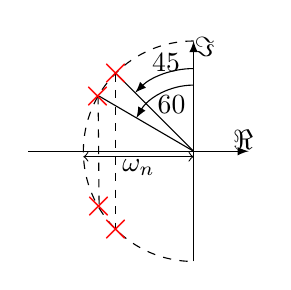
\begin{tikzpicture}[scale=0.7]
			\draw [-latex] (0,2) -- (4,2);
			\draw [-latex] (3,0) -- (3,4);
			\draw [<->] (1,1.9) -- (3,1.9);
			\draw [dashed] (3,4) arc (90:270:2);
			\draw (3,2) -- (1.586, 3.414);
			\draw (3,2) -- (1.286, 3);
			\draw [-latex] (3,3.5) arc (90:135:1.5);
			\draw [-latex] (3,3.2) arc (90:150:1.2);
			\draw [dashed] (1.586,3.414) -- (1.586,0.586);
			\draw [dashed] (1.268,3) -- (1.286,1);
				
			\node [align=center] at (3.9, 2.2) {$\Re$};
			\node [align=center] at (3.2, 3.9) {$\Im$};	
			\node [align=center] at (2, 1.7) {$\omega_n$};
			\node [align=center] at (2.5, 3.6) {$45°$};
			\node [align=center] at (2.6, 2.85) {$60°$};

			\node [align=center, red] at (1.586,3.414) {\Large $\times$};
			\node [align=center, red] at (1.268,3) {\Large $\times$};
			\node [align=center, red] at (1.586,0.586) {\Large $\times$};
			\node [align=center, red] at (1.286,1) {\Large $\times$};
		\end{tikzpicture}
		\caption{Posizione dei poli in catena chiusa per controllo integrale con principio del modello interno.}
		\label{fig:PoliModelloInterno}
	\end{figure}	
	
	
	\subsection{Simulazione e confronto tra modello interno e controllo integrale}
	\label{subsec:SimInterno}
	
		Oltre al principio del modello interno, si è voluto applicare anche il controllo integrale studiato in precedenza. Si confronteranno quindi le prestazioni fra i due controllori sia in simulazione con \textit{SIMULINK} sia in laboratorio con il motore. Si proveranno diversi periodi e ampiezze per il segnale di ingresso e come prestazioni si utilizzeranno l'errore di fase e l'errore di guadagno. Le diverse ampiezze del segnale di riferimento sono $a=10°$, $a=20°$ e $a=50°$, mentre i diversi periodi sono $T_0=1$, $T_0=0.5$, $T_0=0.25$ e $T_0=0.15$ secondi. Come si vedrà a seguire, entrambi i sistemi si comportano abbastanza bene per quanto riguarda l'errore di guadagno, a parte qualche eccezioni nel caso più difficile con ampiezza più grande e periodo più piccolo, mentre vi sono grosse differenze per quanto riguarda l'errore di fase. Per questo motivo si è deciso allora di separare i risultati ragruppandoli per periodi uguali.
		
		\begin{figure}[H]
			\centering
			\includestandalone[width=1\textwidth]{./simulazioni/7_sim_lower_bound}
			\caption{Uscite del motore per periodo $T_0=1$ secondi in simulazione (in linea tratteggiata il riferimento).} 
			\label{fig:simLowerBound}		
		\end{figure}		 
		
		\begin{figure}[H]
			\centering
			\includestandalone[width=1\textwidth]{./simulazioni/7_sim_upper_bound} 
			\caption{Uscite del motore per periodo $T_0=0.15$ secondi in simulazione (in linea tratteggiata il riferimento).}
			\label{fig:simUpperBound}		
		\end{figure}
		
		\noindent Come si vede dalla figura \ref{fig:simLowerBound}, per periodi del senale molto alti, entrambi i sistemi dopo circa un periodo inseguono il riferimento piuttosto bene, fatta eccezione per il controllo integrale che introduce un lieve errore di fase. I problemi  sorgono quando si incrementa la frequenza come in figura \ref{fig:simUpperBound}, il controllo integrale mostra i suoi limiti introducendo sia un grande errore di fase che di guadagno. Il principio del modello interno invece dopo un tempo di assestamento riesce ad inseguire il riferimento solo con un piccolo errore di guadagno trascurabile.	
		
		\begin{figure}[H]
			\centering
			\begin{tikzpicture}[scale=0.61]
			\begin{axis}[
				xscale=1.7,
				yscale=1,
				ylabel={$20\log_{10}P_{ry} \singleSpacing (dB)$},
				y label style={at={(axis description cs:-0.12,.5)},anchor=south},
				xlabel={$\omega \singleSpacing (rad/sec)$},
				x label style={at={(axis description cs:.15,-.1)},anchor=south},
				ytick={-100,-60,...,60},
				yticklabels={$-100$, $-60$, $-20$, $20$, $60$},
				xmode=log,			
				xmin=10,
				xmax=10000,
				ymin=-120,
				ymax=65,
				grid=minor,
				ymajorgrids,
			  	legend style={at={(0.445, 0.98)}, anchor=north east},        
			  	legend cell align=left,     
				legend entries={modello interno, controllo integrale},			
				]
				
			\addplot[red] table {./simulazioni/bode/modello_interno/bode_amplitude.dat};
			\addplot[blue] table {./simulazioni/bode/controllo_integrale/bode_amplitude.dat};
			\end{axis}
			\end{tikzpicture}
			\begin{tikzpicture}[scale=0.61]
			\begin{axis}[
				xscale=1.7,
				yscale=1,
				ylabel={$\angle P_{ry} \singleSpacing (°)$},
				y label style={at={(axis description cs:-0.13,.5)},anchor=south},
				xlabel={$\omega \singleSpacing (rad/sec)$},
				x label style={at={(axis description cs:.15,-.1)},anchor=south},
				ytick={-360,-300,...,0},
				xmode=log,			
				xmin=10,
				xmax=10000,
				ymin=-370,
				ymax=0,
				grid=minor,
				ymajorgrids,
			  	legend style={at={(0.445, 0.98)}, anchor=north east},        
			  	legend cell align=left,     
				legend entries={modello interno, controllo integrale},			
				]
				
			\addplot[red] table {./simulazioni/bode/modello_interno/bode_phase.dat};
			\addplot[blue] table {./simulazioni/bode/controllo_integrale/bode_phase.dat};
			\end{axis}
			\end{tikzpicture}
			\caption{Modulo e fase delle funzioni di trasferimento $P_{ry}$ per modello interno e controllo integrale}
			\label{fig:bode7}
		\end{figure}
		
		 \noindent In figura \ref{fig:bode7} si possono vedere modulo e fase delle funzioni di trasferimento dal riferimento all'uscita dei due tipi di controllo. In particolare si può osservare come il principio del modello interno offre un attenuazione e una fase praticamente nulle per pulsazioni fino circa $100 rad/sec$; ciò vuol dire che segnali fino quella particolare pulsazione potranno essere inseguiti piuttosto bene. Il controllo integrale offre invece queste prestazioni fino a pulsazioni molto minori, soprattutto per quanto riguarda la fase.		
		
		
		
		
		
		
		
	\subsection{Verifica sperimentale in laboratorio}	
	\label{subsec:lab7}	
	
		Le stesse simulazioni sono state ripetute anche con la strumentazione di laboratorio.
	
		\begin{figure}[H]
			\centering
			\includestandalone[width=1\textwidth]{./simulazioni/7_lab_lower_bound}
			\caption{Uscite del motore per periodo $T_0=1$ secondi in laboratorio (in linea tratteggiata il riferimento).} 
			\label{fig:labLowerBound}		
		\end{figure}		 
		
		\begin{figure}[H]
			\centering
			\includestandalone[width=1\textwidth]{./simulazioni/7_lab_upper_bound} 
			\caption{Uscite del motore per periodo $T_0=0.15$ secondi in laboratorio (in linea tratteggiata il riferimento).}
			\label{fig:labUpperBound}		
		\end{figure}
		
		\noindent In figura \ref{fig:labLowerBound} e \ref{fig:labUpperBound} sono riportati gli stessi grafici delle misure fatte in simulazione. Il sistema si comporta grosso modo come quello simulato, ciò che peggiora è l'errore di guadagno alle alte frequenze. Questo può essere dovuto ai limiti fisici dell'apparecchiatura, perché la dinamica del motore non è veloce come ci si aspetta dal modello, ma tutto sommato i risultati dimostrano come il principio del modello interno sia molto adatto per questo tipo di applicazioni.	
	
	